\chapter{Atividades Realizadas}

\section{Protótipo das implementações do método}
\label{primeiroprototipo}
A implementação do método foi toda feita utilizando orientação a objetos em C++, com excessão das funções específicas ao cálculo que possuem implementações, em CUDA, OpenCL e C++. Estas funções específicas ao cálculo consistem de operações básicas com vetores, aproximações para o campo vetorial e o método de Runge-Kutta em si. O código compartilhado entre as demais implementações vai desde as estruturas de dados até representações dos resultados em OpenGL.

O código pode ser encontrado em seu repositório Git \newline(em \href{https://github.com/rafamanzo/runge-kutta}{https://github.com/rafamanzo/runge-kutta}) é organizado basicamente em quatro pastas:
\begin{itemize}
  \item \textbf{core} contém as três implementações do método nas pastas \textit{c}, \textit{cuda} e \textit{opencl}; além das estruturas de dados que repensentam a entrada (\textit{dataset.cpp}) e a saída do método (\textit{fiber.cpp}).
  \item \textbf{example-factories} contém os scripts que geram arquivos de entrada para o protótipo de campos vetoriais sintéticos como exemplos;
  \item \textbf{includes} contém todos os cabeçalhos necessários, facilitando sua inclusão;
  \item \textbf{io} contém as classes que cuidam da entrada e saída do protótipo. A pasta \textit{gui} contém as abstrações utilizadas para a criação de uma interface gráfica com Glut e OpenGL.
\end{itemize}

\newpage
As interações entre todas as classes que compõe o protótipo podem ser vistas através do seguinte diagrama de classes:
\begin{figure}[!h]
  \begin{center}
    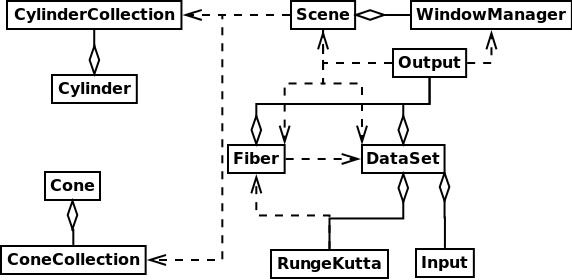
\includegraphics[width=120mm, height=60mm]{images/diagramadeclasse.png}
    \label{fig:diagramadeclasse}
    \caption{Diagrama de classes simplificado para o protótipo}
  \end{center}
\end{figure}

  \subsection{Estruturas compartilhadas em C++}
  A estrutura mais básica é a \textit{vector} contida em \textit{include/dataset.h}, consistindo de três \textit{doubles}. Sua responsabilidade é representar tanto vetores quanto pontos no $\Re ^{3}$. Neste mesmo arquivo também está a representação da classe \textit{DataSet}, cujo uso é representar as informações de entrada referentes ao campo vetorial e encapsular seu acesso. Analogamente, a classe \textit{Fiber} é responsável por representar os resultados da aplicação do algoritmo.
  
  Além destas abstrações de entrada e saída, existem classes que de fato são responsáveis pela entrada e saída do protótipo. A mais simples é a classe que cuida da entrada, \textit{Input}, que possui os métodos para ler um arquivo de texto que contenha as informações sobre o campo vetorial, pontos iniciais e tamanho de passo (conforme descrito no arquivo \textit{README} que acompanha o protótipo). Outra opção de entrada é o formato Analyze que é suportado pelo biblioteca $\textit{CImg}_{\ref{CImg}}$ e portanto o método da classe \textit{Input} que processa este tipo de entrada apenas faz uma chamada a esta biblioteca.
  
  Por fim, a última estrutura compartilhada entre as três implementações é a saída. A forma mais simples de visualizar os resultados é através do $\textit{gnuplot}_{\ref{gnuplot}}$ passando para este o arquivo \textit{rk2-vs-rk4} que é criado ao fim da execução do algoritmo. Por outro lado, a saída pode ser bastante mais complexa que apenas uma classe, como é a entrada, devido à visualização com \textit{Glut} e \textit{OpenGL}.
  
  Esta visualização é composta das classes, aqui denomidas como primitivas, que contém representações de cilindros e cones (classes \textit{Cylinder} e \textit{Cone}) e as responsáveis por representar coleções destas classes (\textit{CyllinderCollection} e \textit{ConeCollection}). Estas classes primitivas contém principalmente informações sobre como renderizar estes objetos.
  
  Por fim, ainda na interface gráfica, existe a classe \textit{Scene} que é responsável por fornecer métodos que utilizam as primitivas para evitar que a classe \textit{WindowManager} use diretamente as primitivas e tenha que conhecer suas especificidades. Ou seja, ela é como uma camada de abstração para a \textit{WindowManager}, permitindo que esta seja responsável apenas pela interação com a \textit{Glut}. 
  
  \subsection{Implementação do método}
  A implementação em cada linguagem pode ser encontrada nas subpastas de \textit{core} (\textit{c}, \textit{cuda} e \textit{opencl}), nos arquivos \textit{rk\_kernel.*} aos quais iremos nos referir apenas como \textit{kernel}. Também cada uma destas pastas contém um arquivo \textit{rk.cpp} reponsável por fornecerer uma interface para seu respectivo \textit{kernel}.
  
  Estas interfaces são utilizadas pois a implementação, por limitação do \textit{CUDA} e do \textit{OpenCL}, não pode ser feita utilizando orientação a objetos. Então a classe (\textit{RungeKutta}) implementada no arquivo \textit{rk.cpp} é a responsável por encapsular o conjunto de funções definidas em seu respectivo \textit{kernel}.

  Cada arquivo de \textit{kernel}, além de conter a implementação do método, possui funções auxiliares para se trabalhar com elementos do $\Re ^{3}$ (soma, subtração, módulo, distância e produto por um escalar) e as funções de aproximação necessárias (\ref{aproximacao}).
  
  Com toda esta estrutura descrita, o método em si é a simples implementação do que é descrito para as ordens 2 e 4 na seção \ref{rungekutta} com especificidades para as diferentes linguagens utilizadas descritas a seguir.
  
  Antes é preciso destacar que todas as implementações de diferentes ordens são funções independentes umas das outras e que, para evitar que falte memória, os resultados foram limitados a 10000 pontos que podem ser gerados a partir de cada ponto inicial.
  
    \subsubsection{Observações sobre o método em C++}
    Esta implementação, ao contrário das demais, foi feita sequencial e apenas não foi feita orientada a objetos para seguir a arquitetura necessária para as outras duas implementações.
    
    \subsubsection{Observações sobre o método em GPU}
    Nestas implementações em CUDA e OpenCL para \textit{GPU}, além do limite de 10000 pontos que podem ser gerados por cada ponto, é feita uma rechecagem após alocar toda a memória necessária para o \textit{DataSet} calculando novamente a quantidade máxima de pontos que podem ser gerados a partir de cada ponto inicial baseado na memória dedicada que restou. Então, o limite é o mínimo entre 10000 e este valor calculado.

    Ainda são checa as características GPU (quantidade de SMs) de forma a alocar toda sua capacidade de processamento sempre que possível. Similarmente é em CUDA checada a quantidade máxima de memória local que cada bloco pode ocupar para garantir que esta não seja excedida. Isto é algo com que o OpenCL já lida sem que o programador tenha que se preocupar.
     
  \subsection{Geração de campos vetoriais sintéticos}
  Campos vetoriais extensos ocupam muito espaço em disco, mesmo, compactados para serem distribuídos de forma prática junto do protótipo. Então, para torna-los disponíveis junto com o protótipo, foram escritos scripts \textit{PHP} que os geram todos eles contidos dentro da pasta \textit{example-factories}.
  
  O campo mais simples gerado possui dimensões 128x128x20, representando uma rotação sobre o eixo z. Nele, o método é aplicado com tamanho de passo 0.1 e pontos iniciais: (0, 16, 10); (0, 32, 10); (0, 48, 10); (0, 64, 10); (0, 80, 10); (0, 96, 10); e  (0, 112, 10). O segundo campo é uma inversão periódica no sentido da coordenada y, num campo de tamanho 512x512x128. A aplicação do método sobre ele se dá com tamanho de passo 0.2 e tem um único ponto inicial: (0, 64, 64).
  
  Os dois campos anteriores são úteis para vrificar se o método se comporta como esperado, mas são pouco úteis para medir a performance e não reproduzem uma variedade de casos. Portanto, os dois exemplos a seguir procuram suprir estas carências.
  
  O terceiro exemplo é um campo com direções aleatórias com dimensão 256x256x256. Para este campo o método é aplicado com tamanho de passo 0.1 e também são criados 256 pontos iniciais com posições aleatórias.
  
  Por fim, no último campo as direções possuem uma distribuição normal com média 10 e variância 1 e sua dimensão é 256x256x256. Ele possui um único ponto inicial aleatório e tamanho de passo 0.1.

\section{Protótipo utilizando a biblioteca VTK}
  Foi utilizada a versão 5.8 da biblioteca VTK (\ref{vtk-5.8}) novamente com C++ para gerar um segundo protótipo equivalente ao anterior (\ref{primeiroprototipo}), capaz de carregar um campo vetorial no formato Analyze e aplicar os métodos de ordem 2 e 4 já implementados na VTK para CPU. Assim, permitindo o planejamento das abstrações necessárias para criar implementações em GPU.
  
  Neste protótipo, muito do código gerado para o primeiro foi reaproveitado. Seu código fonte pode ser encontrado, assim como o primeiro, em seu repositório Git (\href{https://github.com/rafamanzo/runge-kutta-vtk}{https://github.com/rafamanzo/runge-kutta-vtk}).
  
  \subsection{Estrutura}
  A estrutura deste protótipo pode ser entendida como uma simplificação da primeira, contando com apenas 4 classes utilizadas para interagir com as diversas classes da VTK:
  \begin{itemize}
    \item \textbf{AnalyzeReader} é responsável por utilizar a bibliteca \textit{CImg} (também utilizada no primeiro) para ler o arquivo no formato Analyze fornecido na entrada e criar com isto criar uma instância da classe \textit{vtkImageData}, com a qual o VTK poderá trabalhar;
    \item \textbf{Input} recebe os argumentos de entrada e processá-los adequadamente;
    \item \textbf{Tracer} realiza a aplicação do método;
    \item \textbf{Renderer} recebe o resultado da aplicação do método e o exibe na tela já com uma interface que permite escala e rotações.
  \end{itemize}

  As interações entre estas classes e destas com a VTK são ilustradas pelo diagrama de classes simplificado:
  
  \begin{figure}[!h]
    \begin{center}
      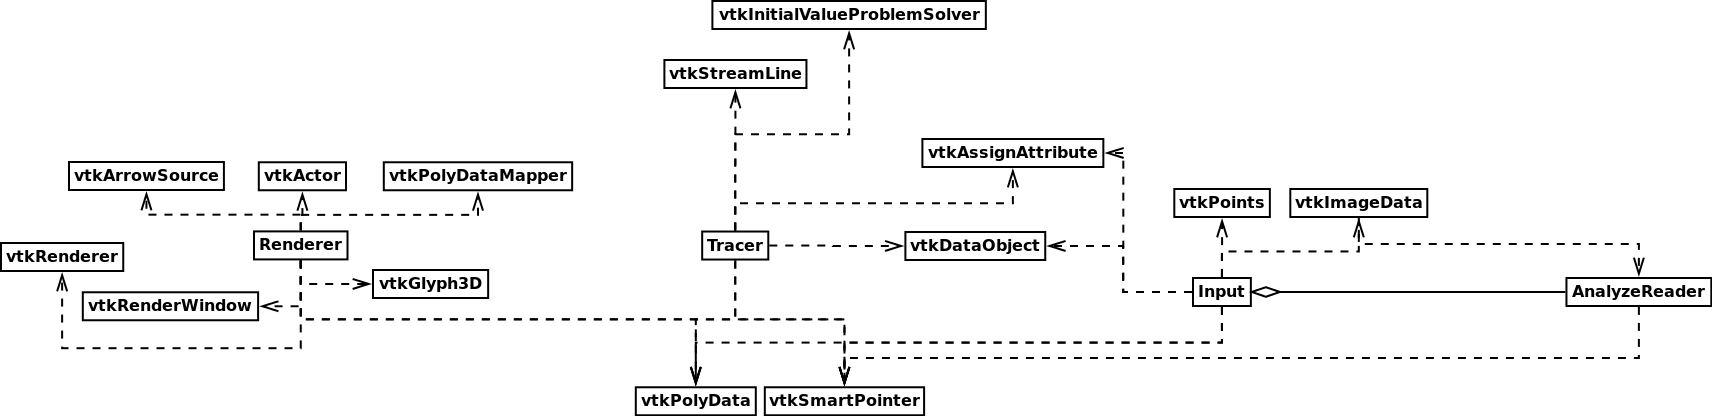
\includegraphics[width=125mm, height=60mm]{images/diagramadeclassevtk.png}
      \label{fig:diagramadeclassevtk}
      \caption{Diagrama de classes simplificado para o protótipo com VTK}
    \end{center}
  \end{figure}
  
  É possível notar que o número de classes necessárias aumentou com relação ao protótipo anterior (\ref{primeiroprototipo}). Porém, boa parte das classes envolvidas neste protótipo são da VTK e apenas as quatro descritas anteriormente tiveram de ser realmente escritas. E mesmo entre estas quatro classes não existe dependência além de uma composição entre a AnalyzeReader e Input.
  
  Isto demonstra que, apesar de utilizar a VTK envolva um número maior de classes sobre as quais o desenvolvedor deve ter conhecimento, ela proporciona um código muito mais enxuto e com baixa dependência entre as classes, representando um protótipo superior em qualidade de código.
  
  \subsection{Planejamento abstrações da VTK para uso de CUDA e OpenCL}
  Basicamente, todo processamento consiste de transferência dos dados dados de entrada à memória, processamento destes dados gerando outros dados de saída e, por fim, a transferência destes dados de saída para a memória.
  
  No caso, o objetivo é possibilitar a aplicação do método em GPU através da VTK. Para tanto, novas implementações das classes da VTK que estejam envolvidas nestas três partes do processamento do método descritas anteriormente. Mais especificamente as classes das quais a classe Tracer depende.
  
  Nesta classe a entrada é recebida em objetos de duas classes da VTK: vtkDataObject (campo vetorial); e vtkPolyData (pontos iniciais). Então, o método utilizado para integração é uma subclasse de vtkInitialProblemSolver para, por fim a classe vtkStreamLine realizar o processamento e devolver a saída em um vtkPolyData. Sendo estas as classes que devem ser abstraídas para GPU.
  
\section{Comparação de perfomance do método entre as implementações em CPU e GPU}
Foram feitas comparações entre as implementações do método para CPU utilizando \textit{POSIX threads} com o método para GPU em CUDA. Estes resultados foram obtidos em duas CPUs Intel e GPUs NVIDIA diferentes a fim de comprovar o que foi afirmado anteriormente sobre os desempenhos do método em cada um destes ambientes.

  \subsection{Metodologia}
    \subsubsection{Dados de entrada}
    Para isto foi gerado um campo vetorial sintético com dimensões de 512 pontos no eixo x, 256 pontos no eixo y e outros 256 pontos no eixo z. Todos com o mesmo vetor direção $(0, 1, 0)$ e até 1024 pontos iniciais da forma $(x, 0, 128)$, onde $0 \leq x \leq 512$ e $z = 128$ ou $z = 129$.
    
    Os testes foram realizados para os primeiros 16, 32, 64, 128 e 256 pontos iniciais a fim de se obter como que o método escala em cada um dos ambientes.
    
    Todo o código utilizado nos testes pode ser encontrado em no repositório git: \href{https://github.com/rafamanzo/runge-kutta-benchmark}{https://github.com/rafamanzo/runge-kutta-benchmark}
    
    \subsubsection{Medições de tempo}
    A medição de tempo é dividida em tempo consumido por operações em memória (alocação e transferência) e processamento do método (operações de ponto flutuante). Sempre realizando a contagem de \textit{clocks} em cada um dos ambientes.
    
    \subsubsection{Casos}
    Cada medição consistiu em executar trinta vezes cada implementação para estes dados (restringindo a quantidade de pontos iniciais conforme descrito). Então, obtendo a média e desvio padrão do tempo em segundos consumidos em operações de transferência de dados, alocação de memória e processamento dos pontos que compõe a trajetória, bem como um histograma.

  \subsection{Resultados em CPU}
  Foram realizados os testes em duas CPUs Intel diferentes:
  \begin{itemize}
    \item Core 2 Duo E7400, com dois núcleos físicos e lógicos a 2.8GHz cada;
    \item Core i7-2620M, com quatro núcleos físicos e lógicos a 2.7GHz cada.
  \end{itemize}
  
  O primeiro utiliza dois módulos de memória DDR2 em Dual Channel, enquanto que o segundo utiliza dois módulos de memória DDR2 em Dual Channel.
    \subsubsection{Runge-Kutta Ordem 2}
    Média dos tempos de execução para processamento em segundos:\\
    \begin{tabular}{| c | c | c | c | c | c |}
      \hline
      \multirow{2}{*}{Processadores}& \multicolumn{5}{|c|}{Quantidade de pontos iniciais} \\ \cline{2-6}
      & 16 & 32 & 64 & 128 & 256 \\ \hline
      Core 2 Duo & 1.182000 & 4.101000 & 17.046000 & 67.923333 & 317.030333 \\ \hline
      Core i7 & 1.693000 & 7.443333 & 34.907333 & 143.061333 & 601.070000\\ \hline

      \hline
    \end{tabular}
    
    \hspace{1mm}\newline
    
    \noindent Desvio padrão dos tempo de execução para processamento em segundos:\\
    \begin{tabular}{| c | c | c | c | c | c |}
      \hline
      \multirow{2}{*}{Processadores}& \multicolumn{5}{|c|}{Quantidade de pontos iniciais} \\ \cline{2-6}
      & 16 & 32 & 64 & 128 & 256 \\ \hline
      Core 2 Duo & 0.044377 & 0.143860 & 0.268398 & 1.632077 & 10.779398 \\ \hline
      Core i7 &  0.095469 & 0.612320 & 0.856380 & 5.185798 & 9.779571 \\ \hline

      \hline
    \end{tabular}
    
    \hspace{1mm}\newline
    
    \noindent Média dos tempos de execução para operações em memória em segundos:\\
    \begin{tabular}{| c | c | c | c | c | c |}
      \hline
      \multirow{2}{*}{Processadores}& \multicolumn{5}{|c|}{Quantidade de pontos iniciais} \\ \cline{2-6}
      & 16 & 32 & 64 & 128 & 256 \\ \hline
      Core 2 Duo & 1.034667 & 1.037000 & 1.046333 & 1.045667 & 1.048667\\ \hline
      Core i7 & 0.946000 & 1.071333 & 1.069667 & 1.049667 & 1.048000\\ \hline

      \hline
    \end{tabular}
    
    \hspace{1mm}\newline
    
    \noindent Desvio padrão dos tempo de execução para operações em memória em segundos:\\
    \begin{tabular}{| c | c | c | c | c | c |}
      \hline
      \multirow{2}{*}{Processadores}& \multicolumn{5}{|c|}{Quantidade de pontos iniciais} \\ \cline{2-6}
      & 16 & 32 & 64 & 128 & 256 \\ \hline
      Core 2 Duo & 0.007180 & 0.009000 & 0.010796 & 0.007608 & 0.008844\\ \hline
      Core i7 & 0.042079 & 0.015217 & 0.009123 & 0.026139 & 0.006000 \\ \hline

      \hline
    \end{tabular}
    
    \subsubsection{Runge-Kutta Ordem 4} 
    Média dos tempos de execução para processamento em segundos:\\
    \begin{tabular}{| c | c | c | c | c | c |}
      \hline
      \multirow{2}{*}{Processadores}& \multicolumn{5}{|c|}{Quantidade de pontos iniciais} \\ \cline{2-6}
      & 16 & 32 & 64 & 128 & 256 \\ \hline
      Core 2 Duo & 1.271000 & 4.013000 & 17.485000 & 68.380000 & 318.383000 \\ \hline
      Core i7 & 1.795333 & 7.721000 & 35.378667 & 144.985667 & 604.026667\\ \hline

      \hline
    \end{tabular}
    
    \hspace{1mm}\newline
    
    \noindent Desvio padrão dos tempo de execução para processamento em segundos:\\
    \begin{tabular}{| c | c | c | c | c | c |}
      \hline
      \multirow{2}{*}{Processadores}& \multicolumn{5}{|c|}{Quantidade de pontos iniciais} \\ \cline{2-6}
      & 16 & 32 & 64 & 128 & 256 \\ \hline
      Core 2 Duo & 0.057175 & 0.469866 & 0.378724 & 1.335073 & 10.443222 \\ \hline
      Core i7 & 0.138558 & 0.460647 & 0.445853 & 1.301178 & 11.964844 \\ \hline

      \hline
    \end{tabular}
    
    \hspace{1mm}\newline
    
    \noindent Média dos tempos de execução para operações em memória em segundos:\\
    \begin{tabular}{| c | c | c | c | c | c |}
      \hline
      \multirow{2}{*}{Processadores}& \multicolumn{5}{|c|}{Quantidade de pontos iniciais} \\ \cline{2-6}
      & 16 & 32 & 64 & 128 & 256 \\ \hline
      Core 2 Duo & 1.034333 & 1.060333 & 1.045333 & 1.048667 & 1.048333 \\ \hline
      Core i7 & 0.982000 & 1.068667 & 1.067333 & 1.051333 & 1.050667\\ \hline

      \hline
    \end{tabular}
    
    \hspace{1mm}\newline
    
    \noindent Desvio padrão dos tempo de execução para operações em memória em segundos:\\
    \begin{tabular}{| c | c | c | c | c | c |}
      \hline
      \multirow{2}{*}{Processadores}& \multicolumn{5}{|c|}{Quantidade de pontos iniciais} \\ \cline{2-6}
      & 16 & 32 & 64 & 128 & 256 \\ \hline
      Core 2 Duo & 0.006155 & 0.048682 & 0.011175 & 0.013350 & 0.007341 \\ \hline
      Core i7 & 0.064570 & 0.010242 & 0.007717 & 0.010242 & 0.014591 \\ \hline

      \hline
    \end{tabular}

  \subsection{Resultados em GPU}
    Foram realizados os testes em duas GPUs NVIDIA GeForce diferentes:
  \begin{itemize}
    \item GTS 450, com 192 CUDA Cores a 1566MHz cada e 1GB de memória GDDR5 à 1804MHz;
    \item GT 520M, com 48 CUDA Cores a 1480Mhz cada e 1GB de memória DDR3 à 800MHz.
  \end{itemize}
  
  De acordo com o fabricante, o primeiro possui performance média para transferência de dados para memória de 57.7GB/s, enquanto que a segunda possui 12.8GB/s.
    \subsubsection{Runge-Kutta Ordem 2}
    Média dos tempos de execução para processamento em segundos:\\
    \begin{tabular}{| c | c | c | c | c | c |}
      \hline
      \multirow{2}{*}{Processadores}& \multicolumn{5}{|c|}{Quantidade de pontos iniciais} \\ \cline{2-6}
      & 16 & 32 & 64 & 128 & 256 \\ \hline
      GTS 450 & 0.049661 & 0.050175 & 0.057119 & 0.057070 & 0.057252 \\ \hline
      GT 520M & 0.054739 & 0.054733 & 0.054850 & 0.061936 & 0.084663 \\ \hline

      \hline
    \end{tabular}
    
    \hspace{1mm}\newline
    
    \noindent Desvio padrão dos tempo de execução para processamento em segundos:\\
    \begin{tabular}{| c | c | c | c | c | c |}
      \hline
      \multirow{2}{*}{Processadores}& \multicolumn{5}{|c|}{Quantidade de pontos iniciais} \\ \cline{2-6}
      & 16 & 32 & 64 & 128 & 256 \\ \hline
      GTS 450 & 0.002440 & 0.000243 & 0.000313 & 0.000089 & 0.000220 \\ \hline
      GT 520M & 0.000033 & 0.000006 & 0.000019 & 0.000264 & 0.000120 \\ \hline

      \hline
    \end{tabular}
    
    \hspace{1mm}\newline
    
    \noindent Média dos tempos de execução para operações em memória em segundos:\\
    \begin{tabular}{| c | c | c | c | c | c |}
      \hline
      \multirow{2}{*}{Processadores}& \multicolumn{5}{|c|}{Quantidade de pontos iniciais} \\ \cline{2-6}
      & 16 & 32 & 64 & 128 & 256 \\ \hline
      GTS 450 & 1.352077 & 1.488127 & 1.776701 & 2.388835 & 3.597740 \\ \hline
      GT 520M & 1.402293 & 1.489929 & 1.680435 & 2.074177 & 2.836108\\ \hline

      \hline
    \end{tabular}
    
    \hspace{1mm}\newline
    
    \noindent Desvio padrão dos tempo de execução para operações em memória em segundos:\\
    \begin{tabular}{| c | c | c | c | c | c |}
      \hline
      \multirow{2}{*}{Processadores}& \multicolumn{5}{|c|}{Quantidade de pontos iniciais} \\ \cline{2-6}
      & 16 & 32 & 64 & 128 & 256 \\ \hline
      GTS 450 & 0.014127 & 0.010570 & 0.013345 & 0.014769 & 0.011500 \\ \hline
      GT 520M & 0.010907 & 0.010067 & 0.011193 & 0.007211 & 0.012150 \\ \hline

      \hline
    \end{tabular}
    
    \subsubsection{Runge-Kutta Ordem 4} 
    Média dos tempos de execução para processamento em segundos:\\
    \begin{tabular}{| c | c | c | c | c | c |}
      \hline
      \multirow{2}{*}{Processadores}& \multicolumn{5}{|c|}{Quantidade de pontos iniciais} \\ \cline{2-6}
      & 16 & 32 & 64 & 128 & 256 \\ \hline
      GTS 450 & 0.089737 & 0.089613 & 0.102665 & 0.102715 & 0.102927\\ \hline
      GT 520M & 0.098342 & 0.098343 & 0.098618 & 0.116622 & 0.164528\\ \hline

      \hline
    \end{tabular}
    
    \hspace{1mm}\newline
    
    \noindent Desvio padrão dos tempo de execução para processamento em segundos:\\
    \begin{tabular}{| c | c | c | c | c | c |}
      \hline
      \multirow{2}{*}{Processadores}& \multicolumn{5}{|c|}{Quantidade de pontos iniciais} \\ \cline{2-6}
      & 16 & 32 & 64 & 128 & 256 \\ \hline
      GTS 450 & 0.000419 & 0.000419 & 0.000263 & 0.000333 & 0.000305 \\ \hline
      GT 520M & 0.000006 & 0.000008 & 0.000037 & 0.000137 & 0.000385 \\ \hline

      \hline
    \end{tabular}
    
    \hspace{1mm}\newline
    
    \noindent Média dos tempos de execução para operações em memória em segundos:\\
    \begin{tabular}{| c | c | c | c | c | c |}
      \hline
      \multirow{2}{*}{Processadores}& \multicolumn{5}{|c|}{Quantidade de pontos iniciais} \\ \cline{2-6}
      & 16 & 32 & 64 & 128 & 256 \\ \hline
      GTS 450 & 1.355632 & 1.490352 & 1.773907 & 2.392552 & 3.599853\\ \hline
      GT 520M & 1.404058 & 1.492534 & 1.675477 & 2.077923 & 2.828944\\ \hline

      \hline
    \end{tabular}
    
    \hspace{1mm}\newline
    
    \noindent Desvio padrão dos tempo de execução para operações em memória em segundos:\\
    \begin{tabular}{| c | c | c | c | c | c |}
      \hline
      \multirow{2}{*}{Processadores}& \multicolumn{5}{|c|}{Quantidade de pontos iniciais} \\ \cline{2-6}
      & 16 & 32 & 64 & 128 & 256 \\ \hline
      GTS 450 & 0.015841 & 0.010029 & 0.010473 & 0.011441 & 0.015122 \\ \hline
      GT 520M & 0.008800 & 0.011051 & 0.009609 & 0.007901 & 0.008453 \\ \hline

      \hline
    \end{tabular}
    
  \subsection{Distribuições}
    Com desvio padrão baixo como o encontrontado, em todos os histogramas a concentração se dá toda sobre a média. Esta característica observada nos desvios padrões também são um forte indicativo de que a média é uma boa estatística para ser utilizada.    
  
  \subsection{Conclusão}
  Os tempos de execução com crescimento exponencial do método em CPU refletem claramente o custo de troca de contexto neste ambiente. Ou seja, a CPU se adapataria melhor a um algoritmo diferente com número fixo de threads igual ao de núcleos físicos do processador. Também no que diz respeito à CPU é evidente o poder de um barramento dedicado para comunicação, onde o tempo gasto em operações na memória praticamente não variou apesar do crescimento exponencial do problema.
  
  \begin{figure}[!h]
    \begin{center}
       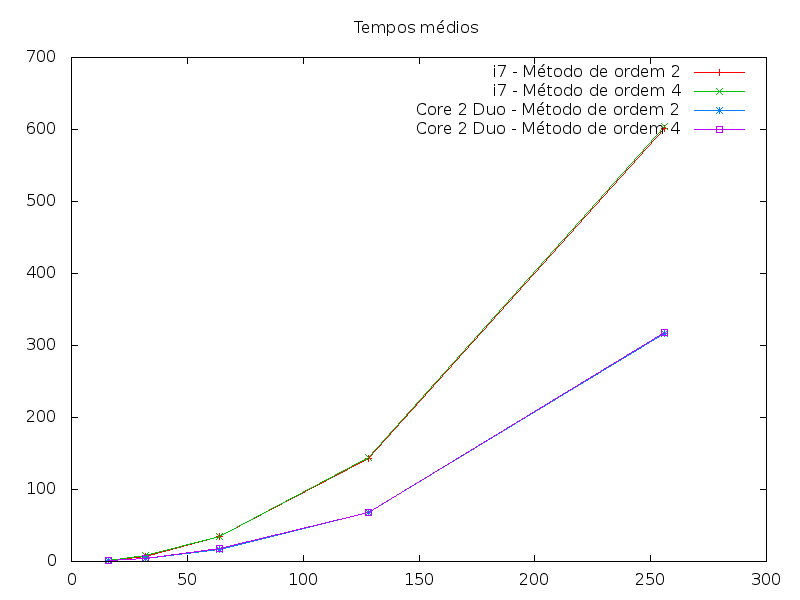
\includegraphics[width=120mm, height=80mm]{images/cpu-means.png}
       \label{fig:cpu-means}
       \caption{Curioso notar que o processador Core 2 Duo bateu em duas vezes um processador Core i7, que é duas gerações posterior ao primeiro.}
    \end{center}
  \end{figure}
  
  Este gráfico ainda nos permite notar que em \textit{CPU} não há diferença prática de tempo entre as ordens apesar de uma realizar o dobro de operações de ponto flutuante. Isto reforça a tese de que o fator limitante para esta implementação em \textit{CPU} é o alto custo da troca de contexto.
  
  \newpage
  Por outro lado, o método em \textit{GPU} obteve tempos de processamento muito inferiores aos de ambas as \textit{CPUs}, em alguns casos chegando à ordem de $10^{-4}$. Porém, a falta de um barramento dedicado causa altos tempos para as operações em memória.
  
  \begin{figure}[!h]
    \begin{center}
       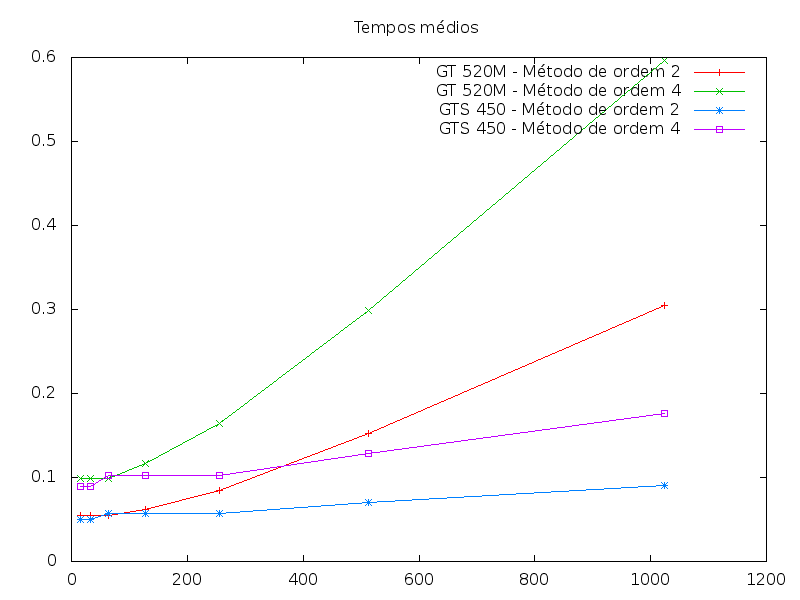
\includegraphics[width=120mm, height=80mm]{images/gpu-means-double.png}
       \label{fig:gpu-means-double}
       \caption{A GTS450 começa a apresentar ganho real de performance a partir dos 256 pontos iniciais, como decorrência do seu maior número de \textit{stream multi-proccessors}}
    \end{center}
  \end{figure}
  
  Este gráfico ilustra um comportmento esperado para GPU, onde no início para um número pequeno de pontos observamos tempo constante, por estar aquém da capacidade do hardware. Então, conforme o problema continua crescendo exponencialmente, o tempo médio começa a crescer, mas linearmente.
  
  \newpage
  O comportamento linear descrito também pode ser observado no que diz respeito às operações de memória.
  
  \begin{figure}[!h]
    \begin{center}
       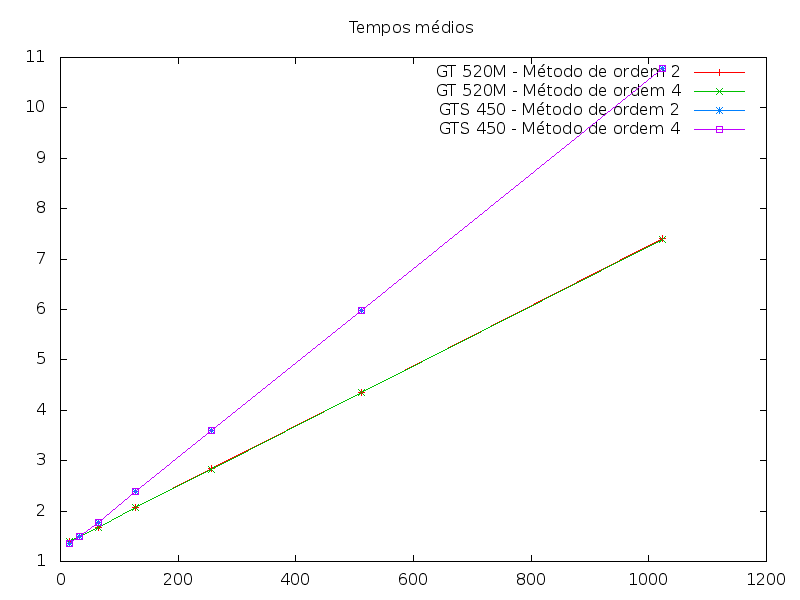
\includegraphics[width=120mm, height=80mm]{images/gpu-memo-means-double.png}
       \label{fig:gpu-memo-means-double}
       \caption{Apesar do tamanho do problema crescer exponencialmente, o tempo gasto para operações de memória cresce de forma linear}
    \end{center}
  \end{figure}
  
  Com estes dados em mãos fica claro que o método em \textit{GPU} não é apenas melhor em comparação com seu equivalente em \textit{CPU}, mas é muito melhor em qualquer para uma quantidade de pontos não muito tão grande (apartir de 64).
  
  Mesmo com um resultado bastante satisfatório, ainda assim, é possível melhorá-lo abrindo mão de precisão e usando a memória \textit{RAM} em conjunto com a da placa gráfica. Para isto, foram feitas novas melhorias e testes com base no método de ordem 4 para a placa GTS 450.

  \subsection{Utilização de precisão simples ao invés de dupla}
  \begin{small}
  Média dos tempos de execução para processamento em segundos:\\
  \begin{tabular}{| c | c | c | c | c | c | c | c |}
    \hline
    \multirow{2}{*}{Precisão}& \multicolumn{7}{|c|}{Quantidade de pontos iniciais} \\ \cline{2-8}
    & 16 & 32 & 64 & 128 & 256 & 512 & 1024 \\ \hline
    Dupla & 0.089737 & 0.089613 & 0.102665 & 0.102715 & 0.102927 & 0.128983 & 0.176045\\ \hline
    Simples & 0.074125 & 0.074505 & 0.074600 & 0.091314 & 0.091356 & 0.092422 & 0.094418\\ \hline

    \hline
  \end{tabular}
  \end{small}  
  \hspace{1mm}\newline
  
  \newpage
  \begin{small}
  \noindent Desvio padrão dos tempo de execução para processamento em segundos:\\
  \begin{tabular}{| c | c | c | c | c | c | c | c |}
    \hline
    \multirow{2}{*}{Precisão}& \multicolumn{7}{|c|}{Quantidade de pontos iniciais} \\ \cline{2-8}
    & 16 & 32 & 64 & 128 & 256 & 512 & 1024\\ \hline
    Dupla & 0.000419 & 0.000419 & 0.000263 & 0.000333 & 0.000305 & 0.000339 & 0.000384\\ \hline
    Simples & 0.000283 & 0.000272 & 0.000272 & 0.000208 & 0.000280 & 0.000336 & 0.000111\\ \hline

    \hline
  \end{tabular}
  \end{small}
  
  \hspace{1mm}\newline
  
  \begin{small}
  \noindent Média dos tempos de execução para operações em memória em segundos:\\
  \begin{tabular}{| c | c | c | c | c | c | c | c |}
    \hline
    \multirow{2}{*}{Precisão}& \multicolumn{7}{|c|}{Quantidade de pontos iniciais} \\ \cline{2-8}
    & 16 & 32 & 64 & 128 & 256 & 512 & 1024 \\ \hline
    Dupla & 1.355632 & 1.490352 & 1.773907 & 2.392552 & 3.599853 & 5.984084 & 10.783370\\ \hline
    Simples & 1.912072 & 2.047864 & 2.327917 & 2.984783 & 4.182320 & 6.618064 & 11.512310 \\ \hline
  \end{tabular}
  \end{small}
  
  \hspace{1mm}\newline
  
  \noindent Desvio padrão dos tempo de execução para operações em memória em segundos:\\
  \begin{tabular}{| c | c | c | c | c | c | c | c |}
    \hline
    \multirow{2}{*}{Precisão}& \multicolumn{7}{|c|}{Quantidade de pontos iniciais} \\ \cline{2-8}
    & 16 & 32 & 64 & 128 & 256 & 512 & 1024\\ \hline
    Dupla & 0.015841 & 0.010029 & 0.010473 & 0.011441 & 0.015122 & 0.016412 & 0.021922\\ \hline
    Simples & 0.010561 & 0.010227 & 0.008126 & 0.016713 & 0.022187 & 0.030160 & 0.081429\\ \hline
  \end{tabular}
  
    \subsubsection{Conclusão}
    Com a precisão simples houve ligeiro ganho no tempo de processamento, mas houve uma ligeira perda no tempo de operações na memória que é a grande limitação desta implementação.
  
  \subsection{Utilização de memória presa}
  \begin{small}
  Média dos tempos de execução para processamento em segundos:\\
  \begin{tabular}{| c | c | c | c | c | c | c | c |}
    \hline
    \multirow{2}{*}{Memória}& \multicolumn{7}{|c|}{Quantidade de pontos iniciais} \\ \cline{2-8}
    & 16 & 32 & 64 & 128 & 256 & 512 & 1024 \\ \hline
    Global & 0.074125 & 0.074505 & 0.074600 & 0.091314 & 0.091356 & 0.092422 & 0.094418\\ \hline
    Presa & 0.074107 & 0.074444 & 0.090507 & 0.107728 & 0.107685 & 0.108624 & 0.110673\\ \hline

    \hline
  \end{tabular}
  \end{small}  
  \hspace{1mm}\newline
  
  \newpage
  \begin{small}
  \noindent Desvio padrão dos tempo de execução para processamento em segundos:\\
  \begin{tabular}{| c | c | c | c | c | c | c | c |}
    \hline
    \multirow{2}{*}{Memória}& \multicolumn{7}{|c|}{Quantidade de pontos iniciais} \\ \cline{2-8}
    & 16 & 32 & 64 & 128 & 256 & 512 & 1024\\ \hline
    Global & 0.000283 & 0.000272 & 0.000272 & 0.000208 & 0.000280 & 0.000336 & 0.000111\\ \hline
    Presa & 0.000230 & 0.000118 & 0.000211 & 0.000266 & 0.000235 & 0.000231 & 0.000273\\ \hline

    \hline
  \end{tabular}
  \end{small}
  
  \hspace{1mm}\newline
  
  \begin{small}
  \noindent Média dos tempos de execução para operações em memória em segundos:\\
  \begin{tabular}{| c | c | c | c | c | c | c | c |}
    \hline
    \multirow{2}{*}{Memória}& \multicolumn{7}{|c|}{Quantidade de pontos iniciais} \\ \cline{2-8}
    & 16 & 32 & 64 & 128 & 256 & 512 & 1024 \\ \hline
    Global & 1.912072 & 2.047864 & 2.327917 & 2.984783 & 4.182320 & 6.618064 & 11.512310 \\ \hline
    Presa & 1.925960 & 2.070551 & 2.380262 & 3.026972 & 4.279094 & 6.787730 & 11.785125\\ \hline
  \end{tabular}
  \end{small}
  
  \hspace{1mm}\newline
  
  \noindent Desvio padrão dos tempo de execução para operações em memória em segundos:\\
  \begin{tabular}{| c | c | c | c | c | c | c | c |}
    \hline
    \multirow{2}{*}{Memória}& \multicolumn{7}{|c|}{Quantidade de pontos iniciais} \\ \cline{2-8}
    & 16 & 32 & 64 & 128 & 256 & 512 & 1024\\ \hline
    Gloval & 0.010561 & 0.010227 & 0.008126 & 0.016713 & 0.022187 & 0.030160 & 0.081429\\ \hline
    Presa & 0.010899 & 0.026004 & 0.016693 & 0.013016 & 0.026585 & 0.024440 & 0.036797\\ \hline
  \end{tabular}
  
    \subsubsection{Conclusão}
    Utilizando a memória presa não houve ganho de performance nos tempos (inclusive houve ligeira perda de performance), porém ainda é um recurso bastante interessante. Isto pois o uso deste recurso faz que ao invés de ser utilizada a memória da placa gráfica seja utilizada a memória principal da máquina. Visto que a memória da placa gráfica costuma ter menos espaço disponível que a memória principal, isto permite o processamento de problemas com concjuntos de dados ainda maiores.
  
  
  \subsection{Avaliação da melhor combinação}
  O primeiro conjunto de testes em GPU nos permite concluir que, de fato, o método de ordem 2 consome metade do tempo acaba consumindo metado do tempo de processamento que o de ordem 4 ao custo de perda de precisão. Porém isto pode ser compensado, quando necessário, aumentando o tamanho do passo do método.
  
  Analisando as melhorias, apesar de  não terem implicado em mais desempenho, o uso de precisão simples e memória presa trouxeram ganhos do ponto de vista do espaço em memória necessário para o processamento do problema, permitindo o processamento de problemas ainda maiores.
  
  O uso de precisão simples reduziu pela metade a quantidade de memória necessária para a resolução do problema, mas, também, ao custo de se perder precisão sobre a resposta. No entanto esta perda será relevante apenas para campos vetoriais bastante complexos e, mesmo neste caso, pode ser compensada quando é diminuído o tamanho do passo do algoritmo novamente.
  
  A memória presa, por sua vez, não reduz o espaço necessário. Ela realiza a alocação na memória principal e deixa esta disponível para a placa gráfica. Com esta mudança no local dos dados o tamanho do campo vetorial suportado aumenta da mesma forma que a quantidade máxima de pontos gerados por cada ponto inicial.
